\subsection{Piivert, a new controller}
To interact with the virtual environment, the author developed an input device called \brand{Piivert} \cite{berthaut2010piivert} shown in \ref{fig:piivert}. This device is separated in two controllers that are properly tied to each hand. This improves the musical control of the user. It combines a 6-\ac{DOF} tracking and high-sensitivity pressure sensing.
The  6-\ac{DOF} tracking allows ray casting and gestures detection. 

The author approach regarding the choice of musical gestures was inspired by Cadoz's \cite{cadoz1999musique} research. Indeed, Cadoz suggested three categories of gestures : selection, modification and excitation gestures. As graphical interaction does not fit to the last category of gestures, the Piivert has an important part in the instrument, thanks to its pressure sensing and vibrating feedback. For instance, excitation can be used to trigger sequences.

\begin{figure}[h!]
\centering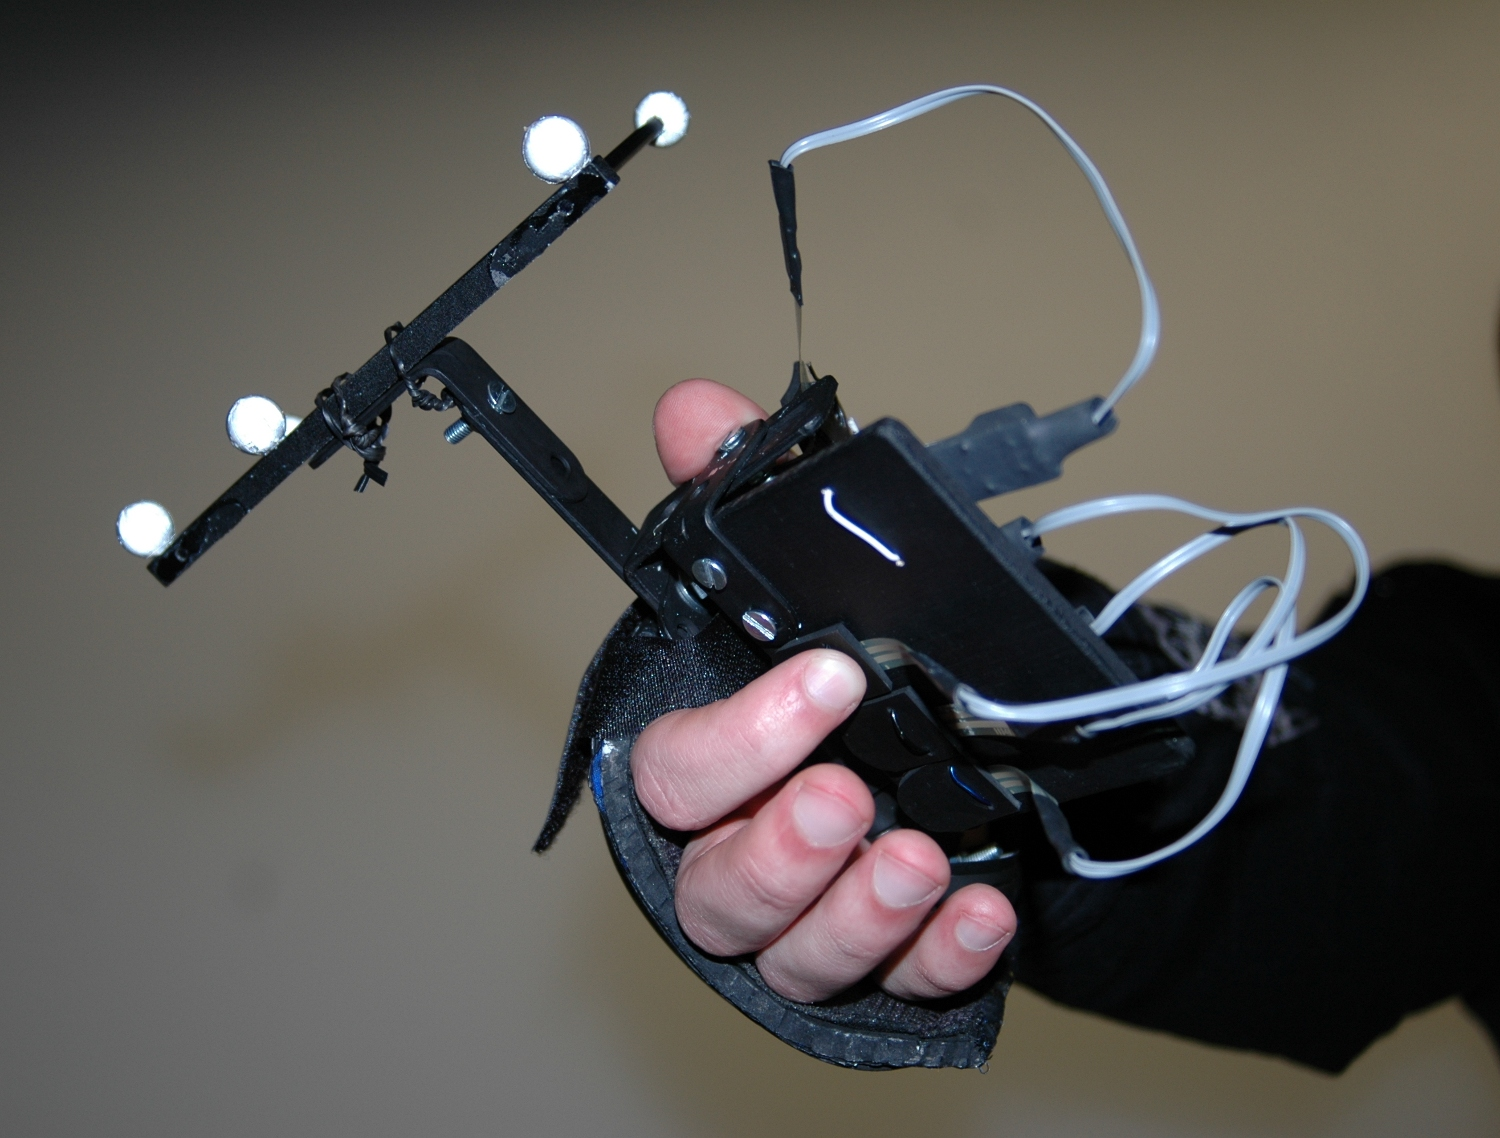
\includegraphics[scale=0.2]{image/piivert.jpg}
\caption{Piivert with pressure buttons on the bottom}
\label{fig:piivert}
\end{figure} 